\documentclass[english]{article}

%% Packages pull in extra commands:
%% http://en.wikibooks.org/wiki/LaTeX/Packages

\usepackage{hyperref}
\usepackage[latin9]{inputenc}
\usepackage[letterpaper]{geometry}
\geometry{verbose,tmargin=1in,bmargin=1in,lmargin=1in,rmargin=1in}
\usepackage{amsmath}
\usepackage{amssymb}
\usepackage{graphicx}
\usepackage{float}
\usepackage{array}
\usepackage{enumerate}
\usepackage{tikz}

% New commands serve as shorthand for frequently used command combinations.
\newcommand{\ind}[1]{\mathbf{1}\left(#1\right)}
\newcommand{\bx}{\mathbf{x}}
\newcommand{\E}{\mathbf{E}}

\title{Fly-by-Logic: User Interface Documentation}
\graphicspath{{./Figures/}} 
\begin{document}

\maketitle
\section{The User Interface}
    
    \begin{figure}[H]
		\label{fig:gui}
        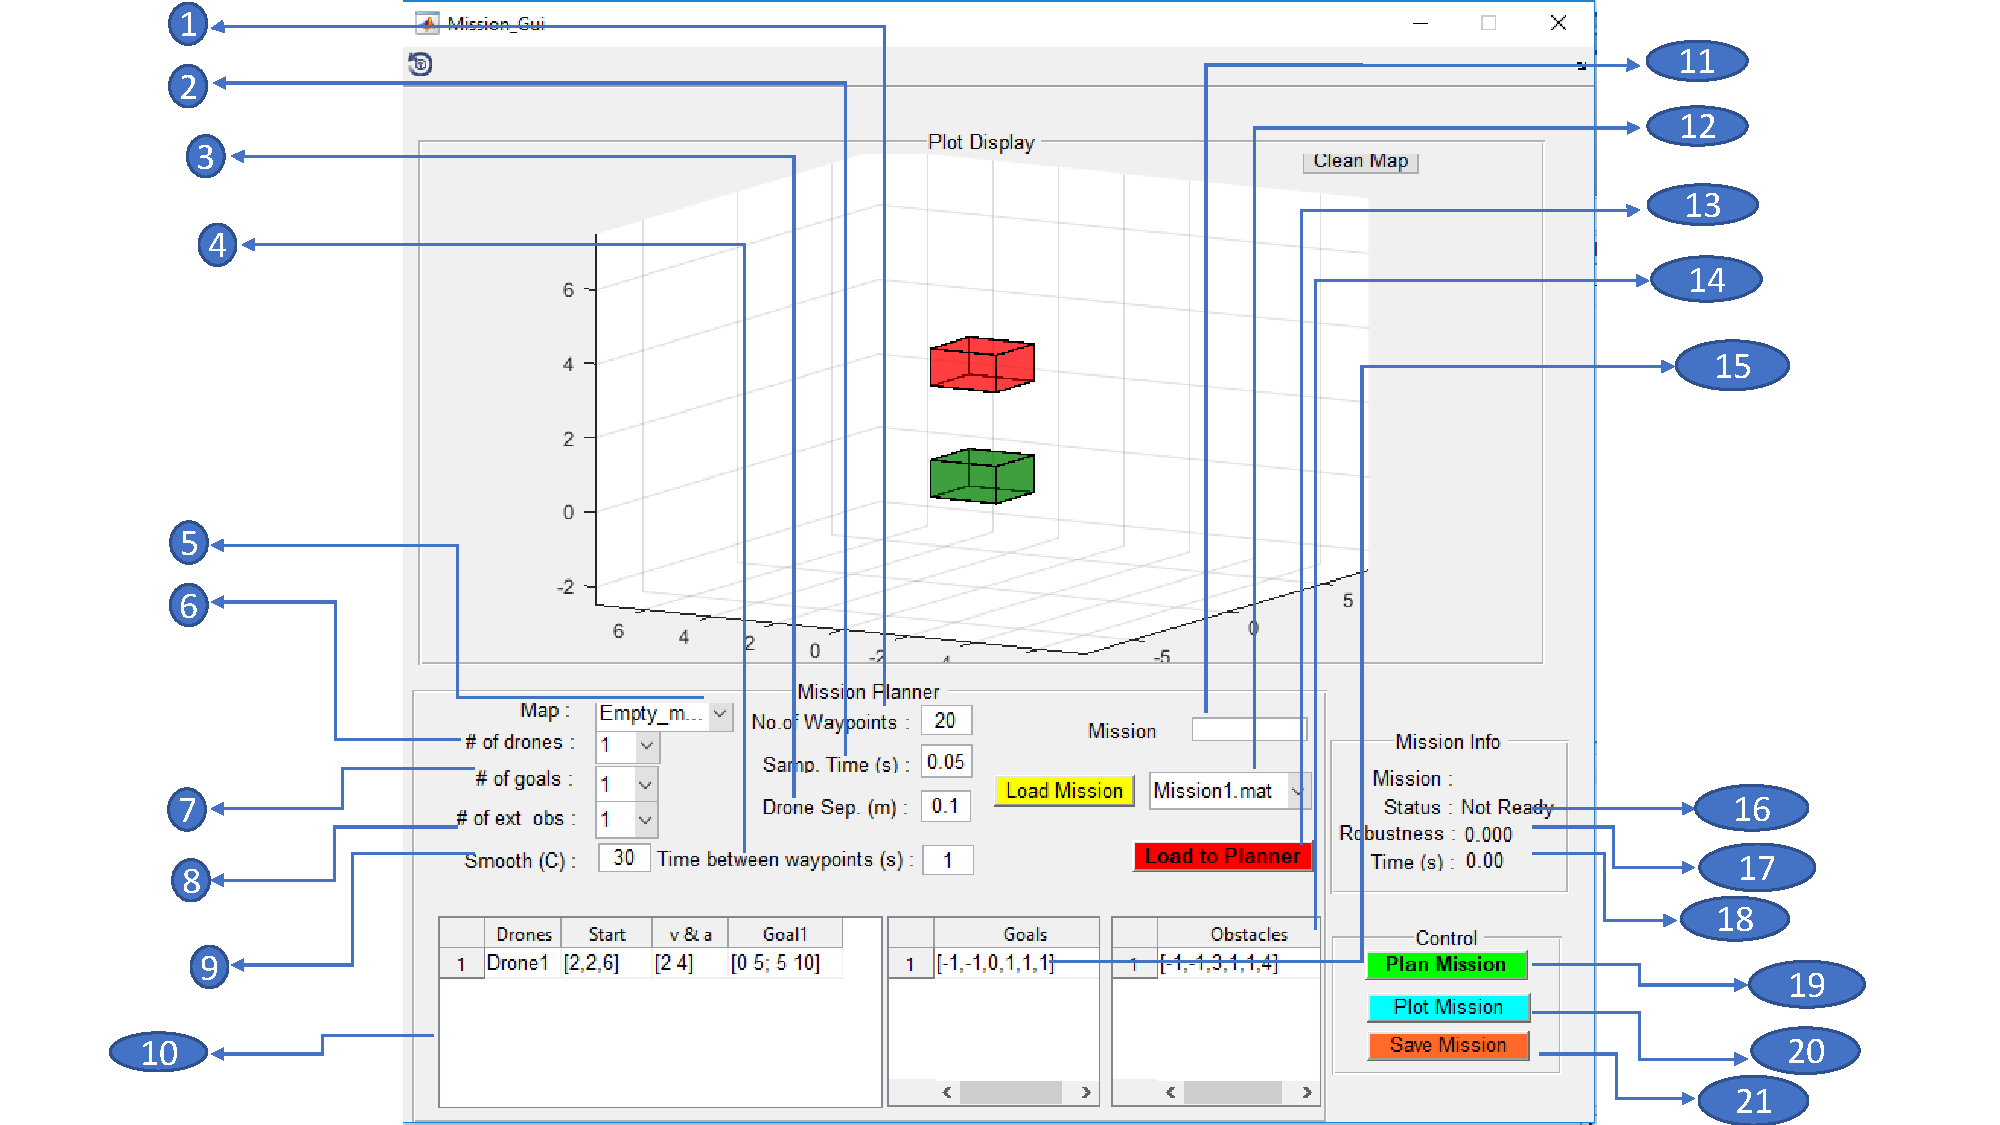
\includegraphics[width=0.99\textwidth]{layout.pdf}
        \caption{The MATLAB Graphical User Interface (GUI) for Fly-by-Logic.}
    \end{figure}

Fig. \ref{fig:gui} shows the user interface through which missions are specified in Fly-by-Logic. Through the interface, the user starts by defining the number of way-points $N$ (same number for each drone), as well well as the (fixed) time, $T$ that the Unmanned Aerial Systems (UAS) take to travel from one way-point to the next. These way-points are the variables that the tool optimizes over, and the overall duration of the mission is then $H=NT$ seconds. Next, the user defines regions in a bounded 3-dimensional workspace (see figure \ref{fig:gui_example}). These regions are axis-aligned hyper-rectangles and can be either \textit{Unsafe} no-fly zones (in red), or \textit{Goal} regions that the UAS can fly to. For each UAS, the user specifies their starting position in the workspace, as well as the velocity and acceleration bounds that their respective trajectories should respect. Finally, the user also specifies the time intervals within which the UAS need to visit some goal sets. 

The components of this are explained in the following text.


\subsection{User interface: Setting mission parameters}

Mission is defined through the following parameters:

\begin{enumerate}
    \item \textbf{No. of Waypoints:} The UAS trajectories that the tool generates are characterized by way-points that are uniformly apart in time, and jerk-minimizing splines between the way-points. The number here sets the number of way-points $N$ (same across all UAS).
    
    
    \item \textbf{Samp. Time (s):} This decides the high-frequency resolution at which the jerk-minimzing trajectories are represented.
    \item \textbf{Drone Sep. (m):} Minimum allowable distance between any two UAS.
    \item \textbf{Time between waypoints (s):} This defines the flight time $T$ in seconds from one way-point to the next, such that $NT$ is the duration of the missions.
    
    \item \textbf{Map:} Loads a text file that defines the workspace. These maps can be designed and saved by the user to load to the planner. 
    \item \textbf{$\#$ of drones} - Number of UAS involved in the mission.
    
    \begin{figure}[H]
        \centering
        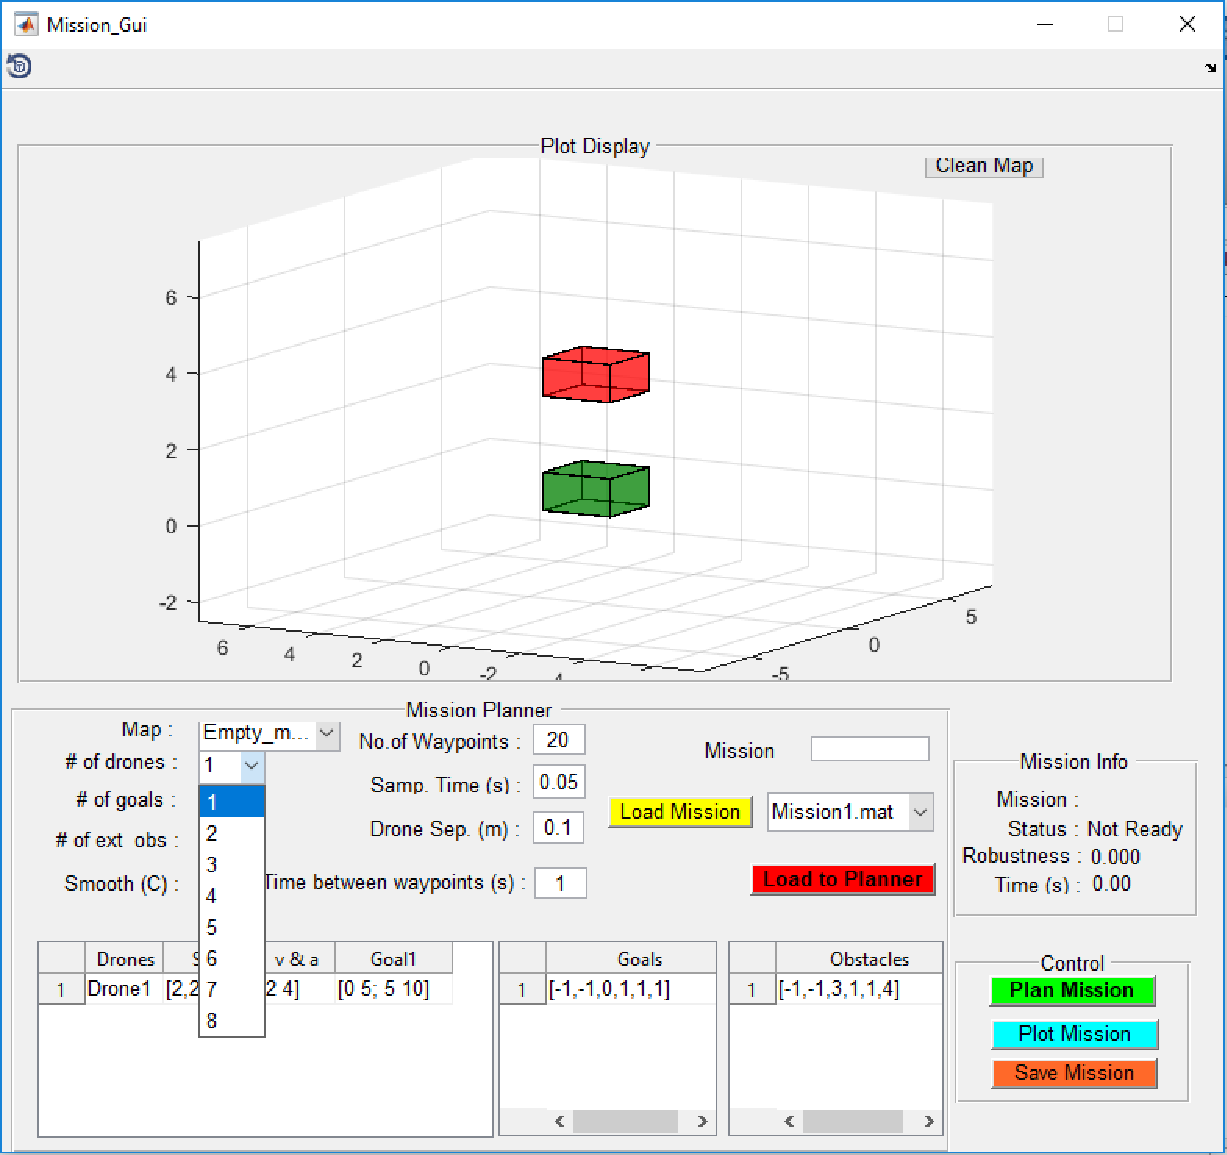
\includegraphics[scale=0.5]{drones.pdf}
    \end{figure}
    \item \textbf{$\#$ of goals} - Number of \textit{Goal} sets for the UAS to visit in the user-defined time interval for a specific mission. 
    \begin{figure}[H]
        \centering
        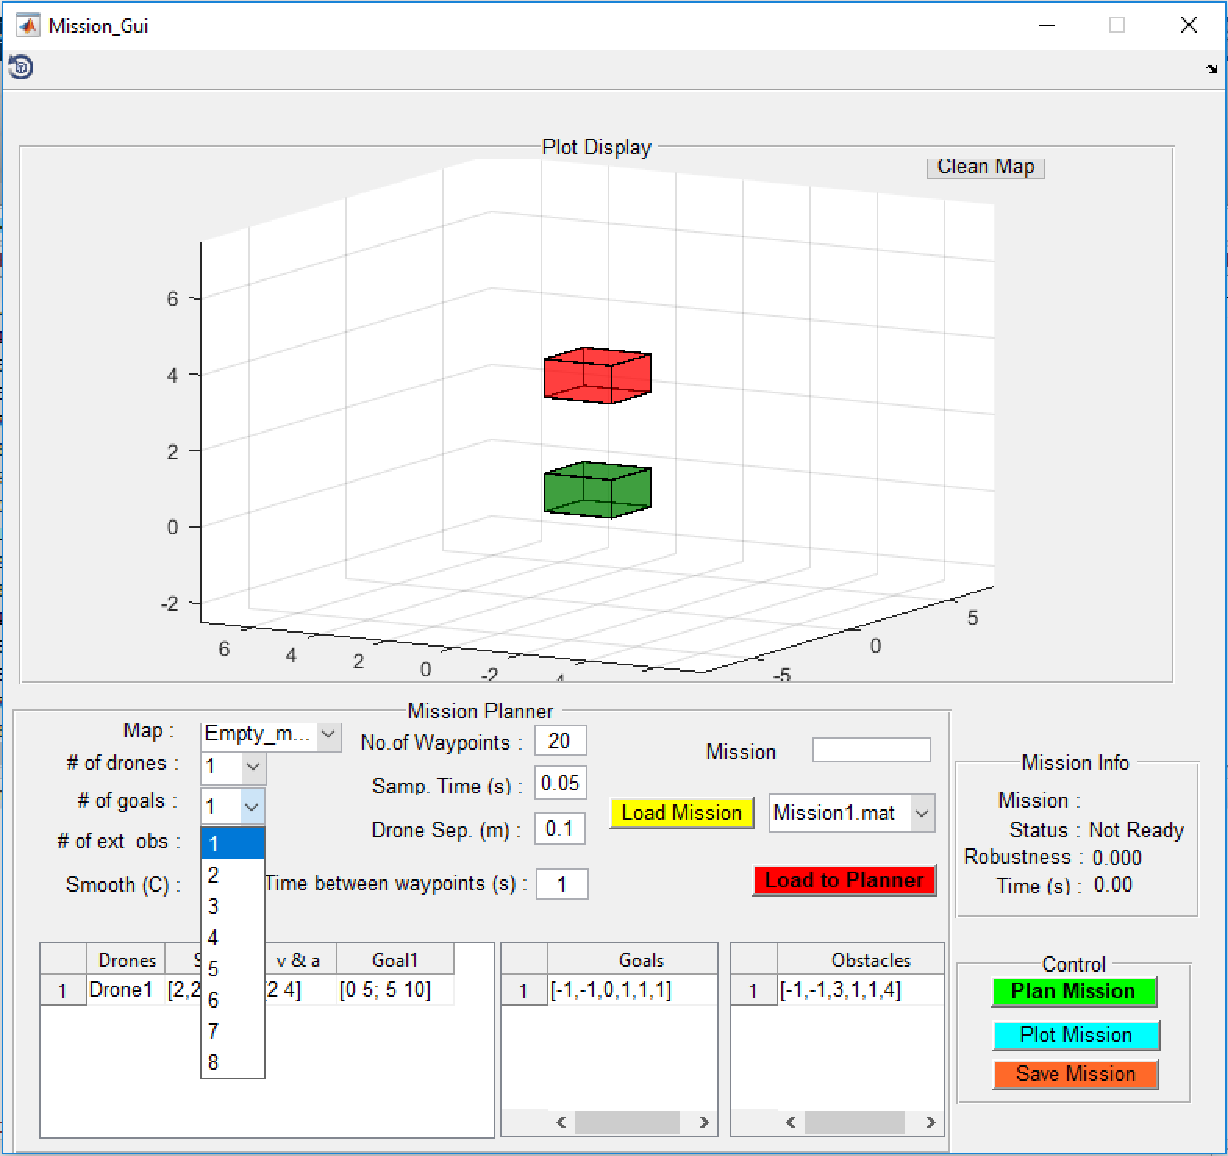
\includegraphics[scale=0.4]{goals.pdf}
    \end{figure}
    \item \textbf{$\#$ of ext obs} - Number of \textit{Unsafe} sets that the drones need to avoid while executing the mission.
    \begin{figure}[H]
        \centering
        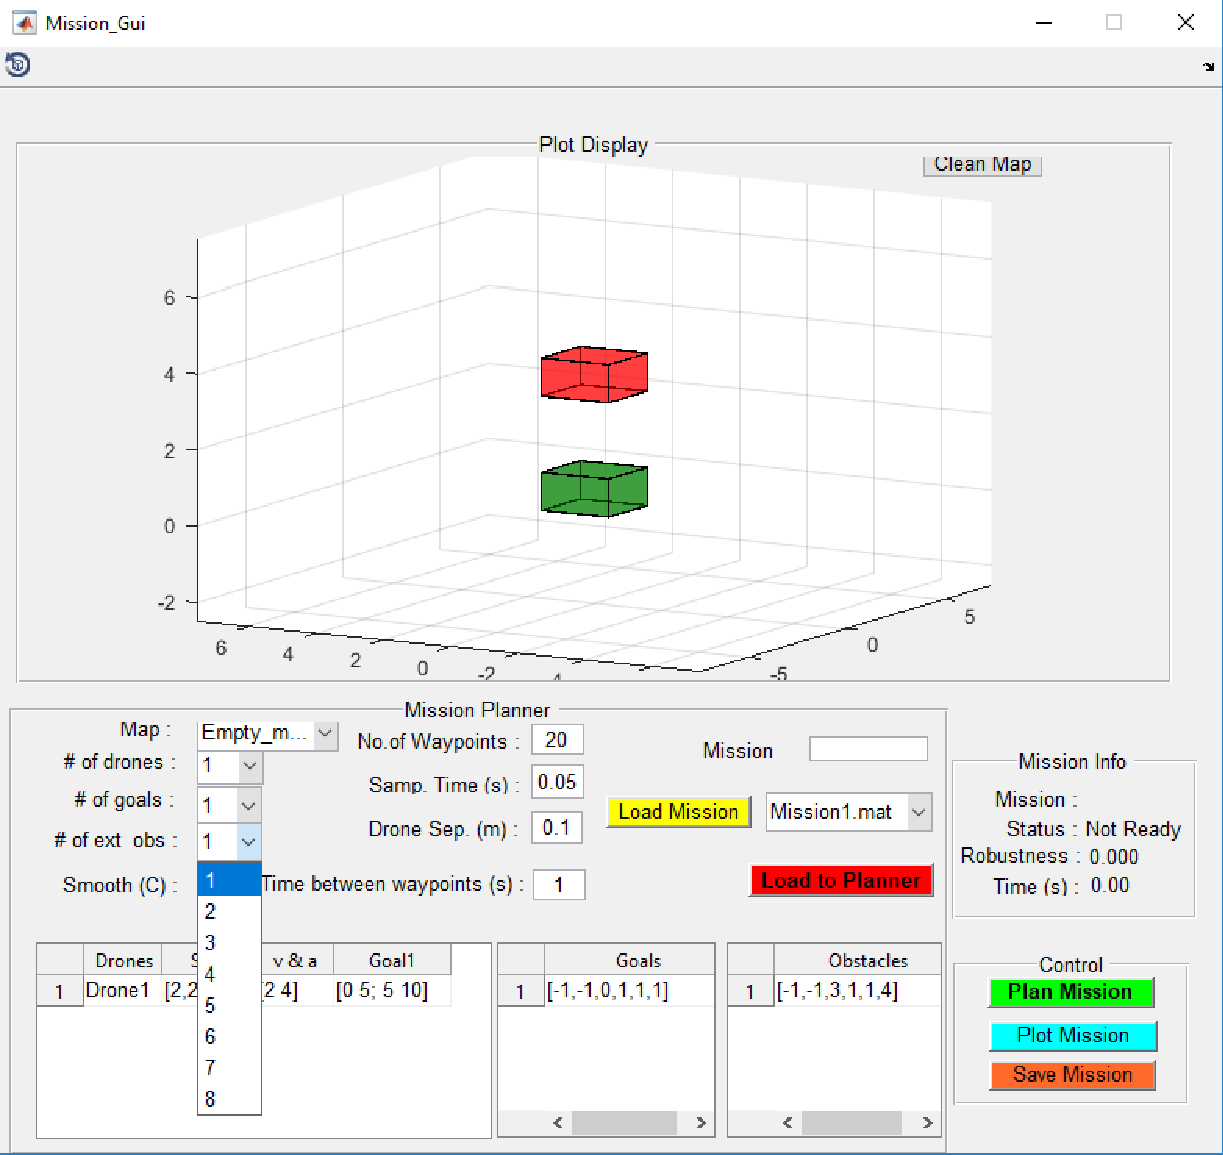
\includegraphics[scale=0.5]{obs.pdf}
    \end{figure}
    \item \textbf{Smooth (C):} A constant that is used to smooth the robustness function to solve the optimization problem. Larger values may lead to numerical instabilities, while smaller values may result in trajectories that do not satisfy the mission.
    
    \item \textbf{Mission Table:} This table defines the UAS specific tasks that define the mission. It has $3+G$ columns where $G$ is the number of \textit{Goal} sets in the mission. The first three columns of the table are \textbf{Drones}, \textbf{Start}, \textbf{v$\And$a}. The Drones column shows the UAS identifier. The Start column contains the start position of the respective drone in the 3-d workspace. This should be in the format \textbf{[x,y,z]}. The  $v\And a$ column gives the velocity and acceleration bounds on the respective UAS such that $|\text{velocity}| \leq v\, \text{ms}^{-1}, |\text{acceleration}| \leq a\, \text{ms}^{-2} \, \forall t \in [0,NT]$ along all 3 axes of motion. These bounds can vary across the all UAS in the mission.
    
The remaining of the $G$ columns define the intervals that the within which respective UAS needs visit the $g^{th},\, g=1,\dotsc,G$ \textit{Goal} set. The format for the time intervals to visit a goal set $G$ is of the form [$tstart_1\, tend_1; tstart_2\, tend_2;\dotsc;tstart_n\, tend_n$]. Here $tstart_i$ and $tend_i$ define the $i^{th}$ time interval for the particular UAS to visit goal set $g$.

Consider an example where the time interval is $[0 5; 10 15]$ and there is one goal. The enforces the requirement that the UAS should visit \textit{Goal} sometime during $0$ to $5$ seconds, and then again within $10$ to $15$ seconds. 

    \item \textbf{Mission:} Sets the name of the custom mission to be saved. After designing a mission, the user can save it by pressing the \textbf{Save Mission} button.
    \item \textbf{Load Mission:} This enables the user to load a previously saved mission.
    \begin{figure}[H]
        \centering
        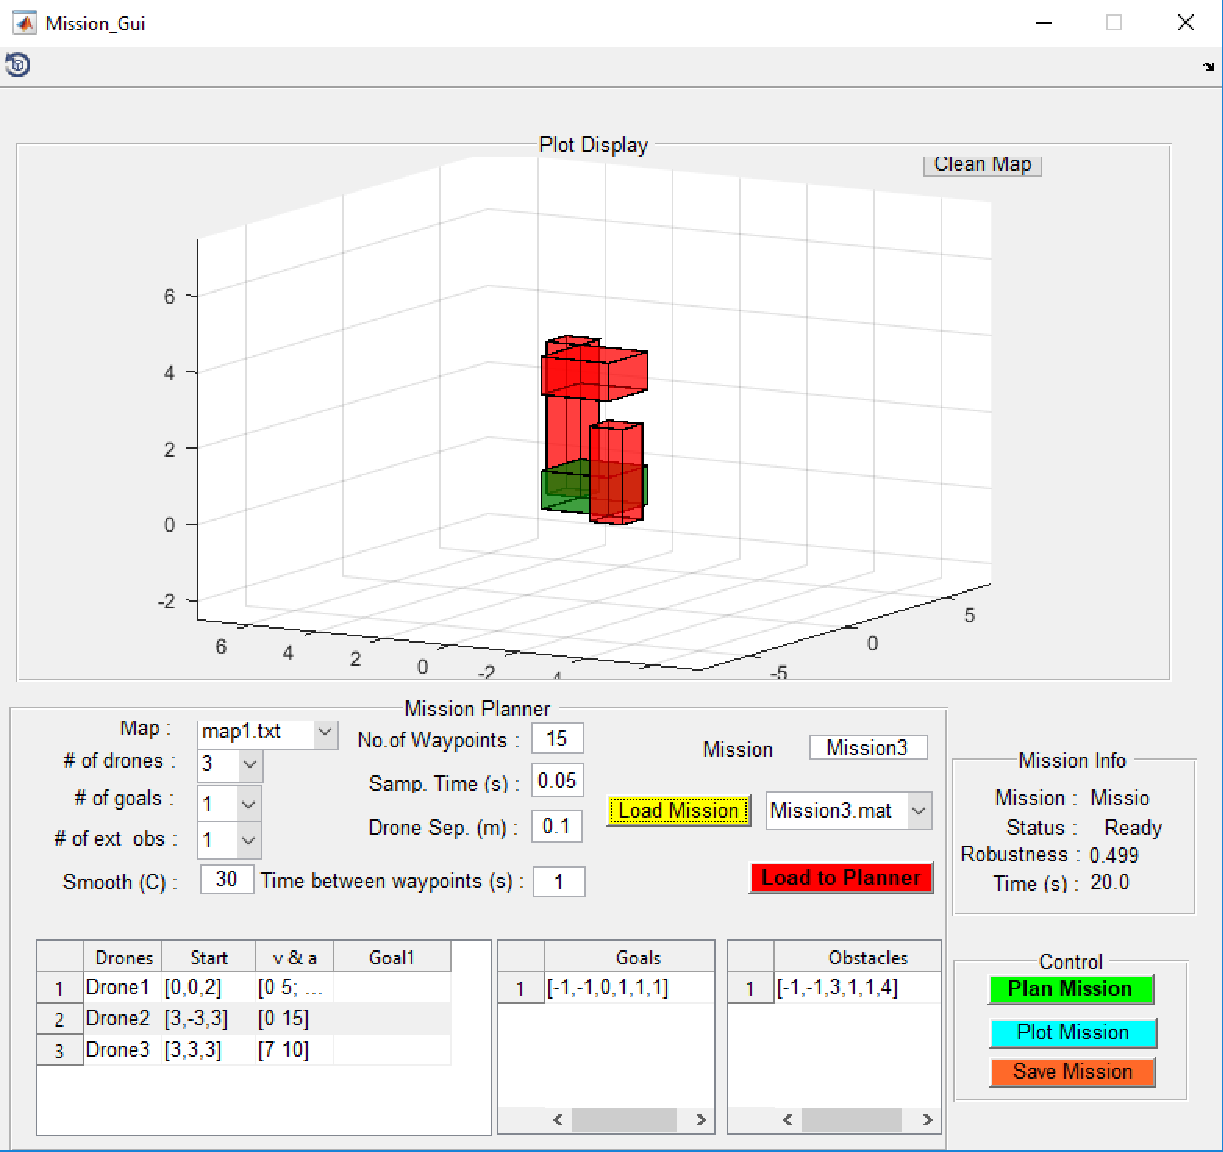
\includegraphics[scale=0.5]{load.pdf}
    \end{figure}
    
    \item \textbf{Load to Planner:}  \textbf{TO BE WRITTEN}
    \item \textbf{Obstacles:} This table gives the lower and upper bounds of the x, y, z coordinates that define the (axis aligned hyper-rectangular) \textit{Unsafe} sets that the UAS must avoid. The number of obstacles are decided by the \textbf{$\#$ of ext obs} parameter. Consider an example where the obstacle is denoted by $[-1,-1,3,1,1,4]$. This implies that the lower bound on the x-coordinate is -1 and the upper bound on x-coordinate for this set is 1. Similarly, the lower bound on y-coordinate is -1, the upper bound on y-coordinate is 1 and lower bound on z-coordinate is 3 and the upper bound on z-coordinate is 4.     
    \item \textbf{Goals:} Similarly, this defines the lower and upper bounds of the x, y, z coordinates of the \textit{Goal} sets which are also hyper-rectangles in 3-d, or a cuboid. The number of Goals by the \textbf{$\#$ of goals} parameter. 
    
    \item \textbf{Status:} This lets the user know if the mission is \textbf{Ready} to be planned. If the user loads one of the saved missions, this parameter lets the user know that the mission is \textbf{Ready} to be planned after the loading has completed. Else, this parameter shows \textbf{Not Ready}
    \item \textbf{Robustness:} This gives the robustness value associated with the planned trajectories after solving the optimization problem which is obtained by Planning the Mission through \textbf{Plan Mission} button. 
    \item \textbf{Time:} This gives a running display of time when the \textbf{Plot Mission} button is pressed to visualize the planned trajectories.
    \item \textbf{Plan Mission:} - This button calls the back-end to generate trajectories to satisfy the mission, once all the parameters to the mission are given to the GUI. 
    \item \textbf{Plot Mission:} This button lets the user visualize the planned trajectories with a real-time playback.
    \item \textbf{Save Mission}: This button lets the user save the mission currently described in the interface. The user can choose to save the mission on a file name which can be given as an input in \textbf{Mission} parameter of the GUI.
\end{enumerate}

\section{Usage}
%\begin{figure}[H]
%        \centering
%        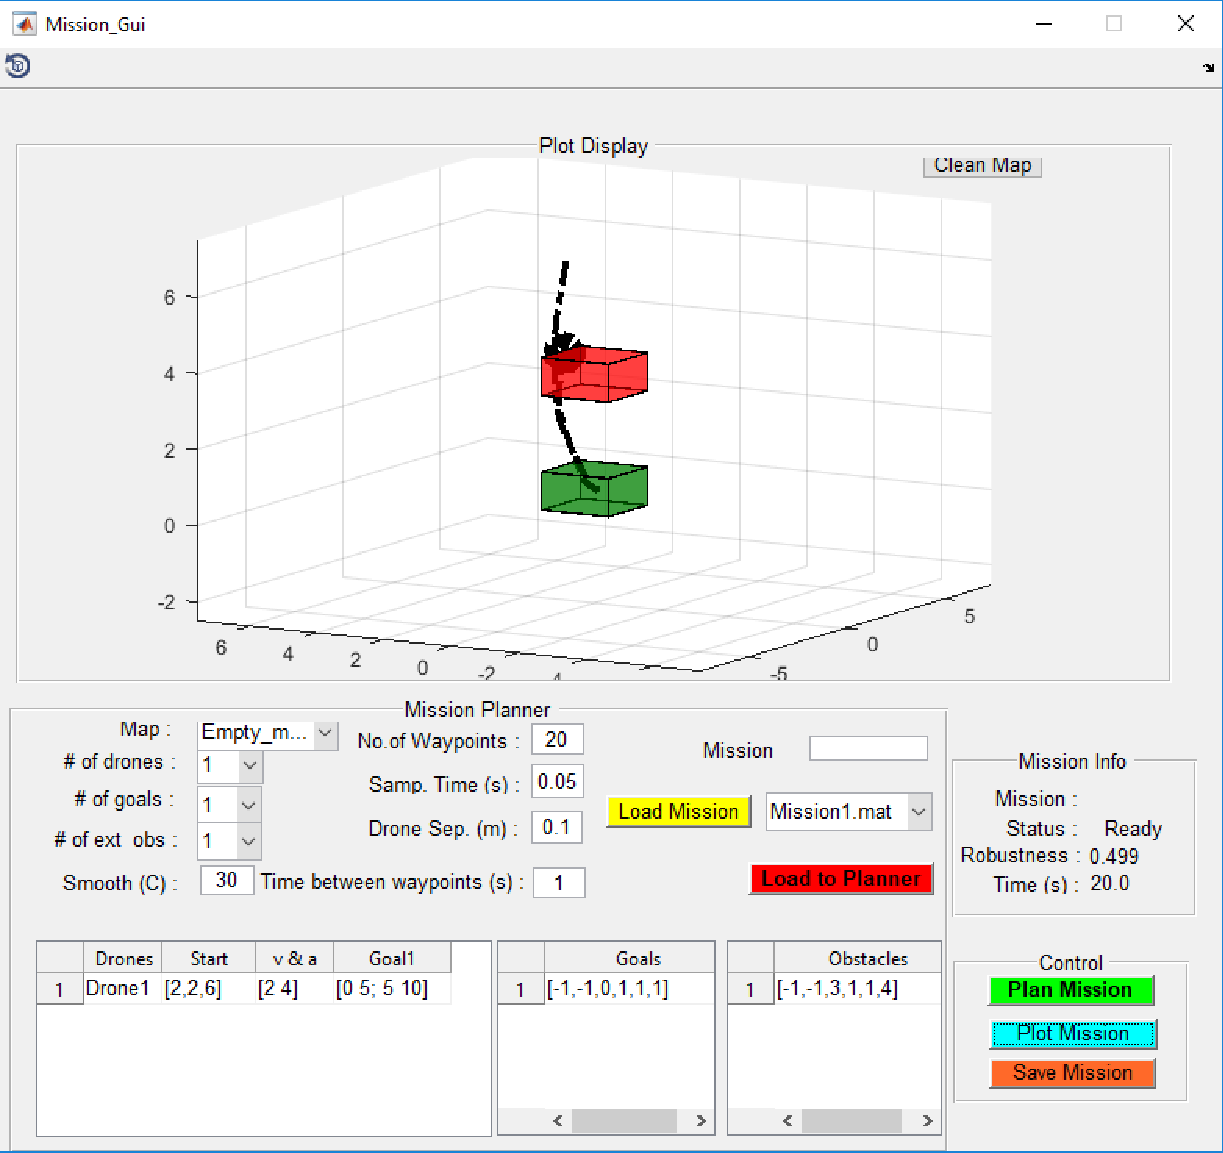
\includegraphics[scale=0.6]{example.pdf}
%    \end{figure}
%
After setting the mission parameters, the user must click the \textbf{Plan Mission} button. Following this, the Fly-by-Logic back-end, runs an optimization to generate trajectories for the UAS in the mission. Once \textbf{Status} changes to Ready, the user can click on \textbf{Plot Mission} to visualize the generated trajectories. 

\end{document}